\documentclass[12pt]{article}
  \usepackage[letterpaper,nohead,left=1.55in,top=1.26in,%
              totalwidth=5.65in,totalheight=8.98in,footskip=0.40in]{geometry}
%  \usepackage[letterpaper,nohead,left=1.51in,top=1.26in,%
%              totalwidth=5.73in,totalheight=8.98in,footskip=0.49in]{geometry}

  \usepackage[dvips]{graphics}
  \usepackage{setspace}
  \usepackage{longtable}
  \setlength{\LTcapwidth}{5.0in}
  \usepackage{subfigure}
  \usepackage{epsfig}
  \usepackage{amsmath}

  \newcommand{\rxn}[1]{\stackrel{#1}{\longrightarrow}}
  \newcommand{\stochrxn}{\emph{stoch\_\-rxn}}
  \newcommand{\tauleaping}{$\tau$-leap\-ing}
  \newcommand{\Tauleaping}{$\tau$-Leaping}
  \newcommand{\vctr}[1]{\mbox{\boldmath $#1$}}
  \newcommand{\mtrx}[1]{\mbox{\boldmath $#1$}}
  \newcommand{\timevec}[2]{\vctr{#1}_{#2}}
  \newcommand{\transpose}[1]{#1^{\mathrm{T}}}
  \newcommand{\matlab}{\textsc{Matlab}}
  \newcommand{\java}{\textsc{Java}} 
  \newcommand{\cpp}{\texttt{C++}}%{\emph{C++}}
  \newcommand{\clang}{\texttt{C}}%{\emph{C}}
  \newcommand{\api}[1]{\texttt{#1}}
  \newcommand{\srccode}[1]{\texttt{#1}}
  \newcommand{\unitqty}[2]{#1\,\mathrm{#2}}
  \newcommand{\ranlib}{\emph{RANLIB.C}}
  \newcommand{\sspack}{\textsc{StochKit}}
  \newenvironment{code}{\begin{quote}\singlespacing}{\end{quote}}

%  \doublespacing

  \setcounter{secnumdepth}{2}
  \setcounter{tocdepth}{\value{secnumdepth}}

\begin{document}
\title{User's Guide for \sspack
\thanks{This work was supported by the California Institute of Technology
under DARPA Award No. F30602-01-2-0558,  by the U. S. Department of Energy
under DOE award No. DE-FG02-04ER25621, by the National Science Foundation
under NSF awards CCF-0326576, CCF-0928912 and ACI00-86061, and by the Institute for
Collaborative
Biotechnologies through grant DAAD19-03-D-0004 from the U. S. Army Research Office.
}
}
\author{ {Yang Cao} \and {Andrew Hall} \and {Hong Li} \and Sotiria Lampoudi \and {Linda Petzold} \\
Department of Computer Science \\ University of Calfornia, Santa Barbara
}

\date{}
\maketitle
\begin{abstract}
Traditional ordinary differential equation-based approaches to
simulation of chemical reacting systems fail to capture the
randomness inherent in such systems at scales common in
intracellular biochemical processes.  A number of stochastic
algorithms have been proposed and implemented on an ad-hoc basis,
but no standard stochastic chemical simulation package exists. We
present \sspack, an efficient, extensible stochastic simulation
framework developed in the \cpp\ language that aims to make
stochastic simulation accessible to practicing biologists and
chemists, while remaining open to extension via new stochastic and
multiscale algorithms. \sspack 1.0 has the basic simulation
ability using the popular Gillespie's SSA algorithm, optimized
SSA algorithm, explicit, implicit, and
trapezoidal tau-leaping methods. Useful tools are provided to make stochastic
simulation more convenient. We provide a Java Converter to convert
an SBML file specifying the chemical mechanism to the input files
needed for our software. We also provide some basic tools to solve
a question of great concern to developers of accelerated
stochastic algorithms---how can we verify the accuracy of a
stochastic solver, given the inherently random nature of
stochastic simulation? The Kolmogorov distance and histogram
distance for quantifying differences in statistical distribution
shapes are provided in the \matlab\ language. For those who need
to run the Monte Carlo simulations a large number of times to
collect the ensemble, we also provide a convenient MPI interface
enabling the Monte Carlo simulation to run on a parallel cluster.
This manual presents a detailed introduction to the software.
\end{abstract}

\newpage
\section{Introduction}
Chemical reaction systems have historically been simulated using
ordinary differential equation (ODE) initial value problem (IVP)
methods.  Such methods appeal to chemical kinetic theory, using
reaction rate constants to characterize the evolution of the system in
time as a function of the concentrations of the reactant species.  As
an example, consider the simple reaction
\begin{equation}
  \alpha S_1 + \beta S_2 \rxn{k} \gamma S_3, \label{eq:intro:ex1}
\end{equation}
where $S_1$, $S_2$, and $S_3$ represent chemical species, $\alpha$,
$\beta$, and $\gamma$ are positive integers denoting the stoichiometry
of the reaction, and $k$ is an experimentally-determined reaction rate
constant expressed in units of concentration per unit time (typically
$\mathrm{mole}\,\mathrm{L}^{-1}\mathrm{s}^{-1}$).

Classically, the simulation of such a reaction would proceed by
writing down the kinetics equations that characterize the
instantaneous rates of change of the concentrations of each species
$S_n$ as a function of the reaction rate $k$, and the
instantaneous concentrations of each of the reactant species
\cite{oxtoby-nachtrieb-90}.  For Reaction
\ref{eq:intro:ex1}, these so-called \emph{reaction rate equations} are:
\begin{eqnarray}
  \frac{d[S_1]}{dt} &=& -k[S_1]^{\alpha}[S_2]^{\beta} \nonumber \\
  \frac{d[S_2]}{dt} &=& -k[S_1]^{\alpha}[S_2]^{\beta} \label{eq:intro:ex1kin} \\
  \frac{d[S_3]}{dt} &=& k[S_1]^{\alpha}[S_2]^{\beta},  \nonumber
\end{eqnarray}
where $[S_n]$ denotes the instantaneous concentration of species
$S_n$ \footnote{The exponents in the reaction rate equations
\eqref{eq:intro:ex1kin} are not always simply the stoichiometric
coefficients of the reaction, because there may be intermediate
species in a reaction whose existence cannot be inferred from the
simplified reaction equation.  In general, we can say $d[S_i]/dt =
f(k, [S_1], \ldots, [S_N])$, where $S_i$ denotes any of the $N$
species participating in the reaction, and $f$ is some differentiable
rational function.  See \cite{oxtoby-nachtrieb-90} for more on the
determination of $f$.}.  Equations \eqref{eq:intro:ex1kin} clearly
constitute a system of coupled first-order ODEs. A standard
initial value problem is formed by specifying the concentration of
each species $S_n$ at some initial time $t_0$.  By applying a
numerical integration algorithm such as Euler's method or any of a
host of Runge-Kutta or multistep methods to the IVP, the concentration
of each species at any future time $t$ can be closely approximated.  A
substantial body of theory exists for the numerical solution of such
IVPs; see for example \cite{ascher-petzold}.

\subsection{The Continuum Approximation}

Two related assumptions are inherent in the use of differential
equations for chemical simulation---first, that the reactant
populations are large, and second, that the reaction environment is
well-stirred.  Indeed, these are the only conditions under which it is
meaningful to discuss the concentrations of the reactant species.
Essentially, these assumptions allow us to approximate the system
state as a smooth, real-valued continuum.  By extension, it is also
assumed that an arbitrary degree of accuracy can be achieved with a
numerical ODE solver by choosing a suitably small step size.

In the context of industrial chemical reactors and other large-scale
domains, the continuum approximation can be quite effectively
employed, and results in no significant loss of accuracy.  However, it
is at best an abstraction---stoichiometry and thermodynamics dictate
that chemical reactions are inherently integer-valued stochastic
processes.  This distinction becomes increasingly important as the
scale\footnote{In this context, scale refers to both the spatial
dimension of the reaction vessel and the populations of the reactant
species.} of the reaction system decreases.


\subsection{Biochemistry and Stochastic Simulation} \label{intro:biochem}

An important class of systems for which the continuum approximation
cannot reasonably be made are those arising in cellular
processes. Biochemical reaction systems are often quite
complex. Reactants may participate in several different reaction
pathways, and may be present in quantities that differ by several
orders of magnitude.  In many cases, the presence or absence of a
single important molecule (i.e., an enzyme) can significantly change
the course of the reaction.  Gene expression is one scenario for which
this is often the case \cite{mcadams-arkin-97, arkin-ross+98,
mcadams-arkin-99}.  When reactant populations are this small (perhaps
in the ones or tens), it makes little sense to speak of their
concentrations, and the standard ODE/IVP numerical simulation
techniques are no longer applicable.  Clearly an alternative approach
is called for.

Because chemical reactions result fundamentally from random collisions
of discrete molecules, a more faithful numerical simulation technique
might try to explicitly model these molecular interactions.  Rather
than tracing the evolution of the concentration of each species in
time by approximating it as a differentiable function, such methods
would instead tally the number of molecules of each species, and rely
on discrete-event simulation techniques to evolve the population
vector in time.

An important advantage of the discrete approach to modeling chemical
reaction systems is that it is capable of capturing the randomness
inherent in such processes.  Because the populations of important
species can be quite small, the evolution of the system state may
depend strongly on the relatively unlikely interaction of these
molecules with those of other, more abundant species.  Such an
interaction can result in a cascade of other reactions that
significantly alters the system state.  In a very real sense, the
state of such a system at any time $t > t_0$ depends not only on the
relative abundance of each of the reactant species at the initial time
$t_0$, but on the exact position, velocity, orientation, etc.\ of
\emph{each~molecule} at that time.

For a variety of reasons, this sensitive dependence on initial
conditions presents a problem.  Quantum mechanics (specifically the
Heisenberg Uncertainty Principle) asserts the impossibility of ever
measuring the exact position and velocity of a single particle, to say
nothing of an entire system of hundreds or even millions of molecules.
Furthermore, even if it were theoretically possible to do so, so much
initial data would be needed that the simulation would be impractical
to use.

Stochastic methods offer a convenient shortcut that allows us to avoid
the initial condition dilemma.  Rather than employing an exact
physical model to track the movement and interactions of each
molecule, we can instead use a probabilistic model that estimates the
likelihood of occurrence of each reaction pathway as a function of the
instantaneous population of each reactant species and a rate
constant $c$, derived from the standard reaction rate
constant $k$\cite{Gillespie76}.  
We can then draw samples from these probability
distributions using standard Monte Carlo techniques to determine the
time of the next reaction event, and update the system state according
to the stoichiometry of that reaction.  Gillespie's \emph{Stochastic
Simulation Algorithm} (SSA) \cite{Gillespie76, Gillespie77} is the
seminal work in this direction (for a detailed description of the SSA,
see \cite{Gillespie76, Gillespie77}). By performing a large number of
realizations (and with a sufficiently good random number generator),
such stochastic techniques make it possible to visualize the entire
distribution of possible system states at time $t$.

\subsection{Accelerated Stochastic Methods}

Unfortunately, the rigorous physical basis for the SSA comes at a high
cost in computational run-time, as these algorithms derive their
accuracy from the explicit modeling of each reaction event.  Even
systems with relatively modest reactant populations and reaction rates
might generate millions of such events in a short time, and the number
of events tends to increase superlinearly as the population size increases.
Furthermore, biological reaction networks frequently feature some
pathways with comparable forward and reverse rates that are large
relative to those of the other pathways.  These systems effectively
involve multiple time scales, with uninteresting high-frequency
oscillations superimposed on a slow overall trend driven by the more
important reaction channels.  In such cases, the vast majority of the
simulated reaction events will consist of forward and reverse firings
of these uninteresting channels, resulting in relatively little change
to the overall population vector.  If we are concerned with the
distribution of the population at some final time $t_f$ rather than
with the exact sequence of reactions that occurred in a particular
realization, much of the computation time is wasted on `uninteresting'
reaction events.

Accelerated stochastic methods are an active area of research in
computational biochemistry.  These algorithms seek to improve upon the
performance of the SSA by enabling larger time steps, sacrificing some
accuracy in the name of efficiency.  Various methods have been
proposed (see \cite{Gillespie01, rao-arkin-02, SPEA1, SPEA2,
frankowicz-moreau+93}, for example), each with a different
strategy for relieving the computational burden of simulating each
reaction event.  Such techniques appear quite promising, often
decreasing the runtime by several orders of magnitude while
maintaining a high degree of accuracy.  However, no `silver bullet'
has thus far been discovered. Conditions that will cause each
technique to fail outright or rapidly to lose accuracy are known.
Accelerated stochastic simulation techniques will likely continue to
be an important area of research until a suitably robust and
efficient, multiscale algorithm is developed.


\subsection{Scope of Work}

The work presented herein consists of a suite of software tools
for stochastic chemical simulation developed for the \cpp\
\cite{c++}, \java\ \cite{java} and \matlab\ \cite{matlab}
programming languages. The intended audience for the programs can
be divided into two distinct, yet equally important groups---those
doing research on and development of stochastic simulation
methods, and those seeking to employ such methods to further their
biological or chemical research.

The primary tool presented is a generalized stochastic simulation
package \sspack. This package makes it possible
to access a variety of stochastic solver algorithms through a unified
interface, such that any available solver can be applied to a given
problem by changing a single function parameter.  In addition, due to
the modular nature of the package, those developing new solver
algorithms (or simply refining existing ones) need only supply a new
routine that captures their particular innovation (i.e. stepsize
selection, single step execution, data management, etc.).

A number of secondary tools are provided to complement the
stochastic simulation solvers. The DataAnalyzer assists with
collecting and analyzing distribution statistics generated by making
ensemble runs of the solver on a given problem.  These tools are
useful for comparing the accuracy of various solver algorithms, and
for visualizing the range of outcomes a particular problem can
generate. The SBML2StochKit Converter provides a tool to convert an
SBML \cite{sbml} file to the input files required by \sspack. Using
this converter, the user can conveniently construct their problem files
using any SBML constructor and run the simulation using \sspack.
In many applications, Monte Carlo simulation has to be run a large number of
times to collect the ensemble. This work is natural for parallel computing.
We provide an MPI interface to the StochKit package. The user can easily
use this tool to collect the ensemble using a parallel cluster.
Thus, \sspack \ and its supporting tools should be effective and easy to
use for both of its intended audiences.

The structure of \sspack \ is shown as in Figure \ref{code_structure}.
In this manual we will explain the details of each block.

\begin{figure} \label{code_structure}
\vspace{11pt}
\centerline{\psfig{figure=sspackstructure.eps,width=5in}}
\caption{Structure of \sspack}
\vspace{11pt}
\end{figure}

\section{Mathematical Primitives in \cpp} \label{cpp_implementation}

\sspack \ was initially developed in the \matlab\ language\cite{Hallthesis}.
The development of the \cpp\ implementation of \sspack \
was slowed by the low level of support for scientific
programming provided by the \cpp\ standard library.  Specifically,
matrix and vector primitives are not built into the language, though
the strong support for data abstraction and operator overloading make
it relatively easy to create linear algebra libraries whose syntax and
semantics closely match those of standard mathematical notation.  A
number of commercial (\cite{roguewave}) and open-source (\cite{MTL,
TNT, blitz++, POOMA, lapack++}) libraries provide this capability
already.

A review of the freely available linear algebra libraries for \cpp\
was inconclusive.  LAPACK++ (\cite{lapack++}) seemed like a logical
choice due to its affiliation with the successful LAPACK
Fortran/\clang\  libraries \cite{lapack}, but it has been superseded by TNT
(\cite{TNT}), which appears to be no longer supported.  MTL
(\cite{MTL}), Blitz++ (\cite{blitz++}), and TNT (\cite{TNT}) were
rejected for syntactical reasons---although improved performance is
the primary goal of the \cpp\ implementation, a secondary goal is to
maintain as much syntactic commonality with the \matlab\
implementation as is feasible.  For this reason, it was decided that
it would be worthwhile to spend some time implementing a small library
whose syntax and semantics conformed to those of \matlab.  This
decision was made with some trepidation, and will be worth revisiting
in the future if a ``standard'' \cpp\ linear algebra library emerges.

\subsubsection{Basic Capabilities}

The CSE::Math library defined and implemented in the {\it Math} directory
provides a set of operations to ease the transition from \matlab\
to \cpp\ development. It is not intended to serve as a
general-purpose high-performance linear algebra library,
but rather to minimize surprises for experienced \matlab\ programmers while
remaining as efficient as possible within the context of \sspack.
The basic capabilities are outlined below.
\begin{description}

  \item[Vector and (dense) Matrix Classes] Basic linear-algebraic
  quantities are implemented with strict deep-copy.  This means that
  unnecessary memory allocation and data movement may sometimes occur,
  but guarantees that modifications to one vector or matrix do not
  inadvertently cause changes in others via aliasing.  Vectors and
  Matrix are implicitly column-oriented. This helps to construct internal
  calls to the popular linear algebra Fortran packages (LAPACK or LINPACK)
  when necessary. The \srccode{Vector} and \srccode{Matrix} classes and
  all of the following operations are
  defined in the \srccode{CSE::Math} namespace.

  \item[Indexing Operations] Elements from vectors and matrices can be
  accessed using the `\srccode{()}' operator as in \matlab.  Unlike
  \matlab, indices start at 0 (as is customary in \clang\  and \cpp).
  Rows and columns of matrices can be selected using the \api{Row()}
  and \api{Col()} member functions.  This is a necessary departure
  from the \matlab\ slicing syntax, as the `\srccode{:}' operator is
  not available for overloading in \cpp.  These operations return
  objects that serve as proxies for the row or column of the original
  matrix, such that the expression `\srccode{m.Row(0) = 1;}' fills the
  top row of the matrix with ones, rather than creating a separate
  vector object and filling it with ones.  However, all operations
  defined for vectors are also defined for matrix row and column
  proxies, so they can be treated as vectors when convenient without
  excessive data copying.

  \item[Scalar-Vector and Scalar-Matrix Operations] As in \matlab,
  binary operators `\srccode{+}', `\srccode{-}', and `\srccode{*}'
  involving any mix of scalar and vector or scalar and matrix operands
  are provided.  The resulting value is a matrix or vector equal to
  the original with the scalar operation applied to each element.
  Thus, the expressions `\srccode{y = x * 5;}' and `\srccode{y = 5 *
  x;}' (where \srccode{x} and \srccode{y} are vectors) are equivalent,
  with the result that $||\texttt{y}|| = 5 ||\texttt{x}||$.  The division
  operator, `\srccode{/}', can have a vector or matrix on the left
  side and a scalar on the right, and similarly applies the scalar
  division to each element of the matrix.  In addition, the
  `\srccode{+=}', `\srccode{-=}', `\srccode{*=}', and `\srccode{/=}'
  operators are provided for vector or matrix left sides, and result
  in in-place modification of the left side operand.  Thus,
  `\srccode{x += 5;}' is semantically equivalent to `\srccode{x = x +
  5;}', but avoids the expensive creation of a temporary object to
  hold the intermediate result.  These operators have no analog in
  \matlab, but will be familiar to \clang\  and \cpp\ programmers and
  are provided because they are significantly more efficient when
  applicable.

  \item[Vector-Vector Operations] Vectors can be added and subtracted
  just as in \matlab.  An \api{InnerProduct()} function is provided to
  obviate the need for a data-copying transpose operation (although
  Matrix objects do have a defined \api{Transpose()} function).  The
  \api{Norm()} function can compute any vector p-norm. As mentioned above, all
  vector operations are equally valid for matrix row and column proxies.

  \item[Matrix-Vector Operations] Vectors can be left-multiplied by
  matrices, and linear systems can be solved for a particular right
  side vector using the \api{SolveGE()} function. If the USELAPACK option is
  chosen, \api{SolveGE()} internally calls LAPACK Fortran LULinearSolver
  dgesv(), otherwise we provide a simple implementation of Gaussian
  Elimination with partial pivoting. Our numerical test shows that the
  LAPACK function is 10\% slower but should be more robust.

  \item[Matrix-Matrix Operations] Matrices can be added, subtracted,
  and multiplied using standard operator syntax.  An identity matrix
  of any size can be constructed via the \api{Identity()} function,
  and the \api{Zeros()} and \api{Ones()} functions are analogous to
  the \matlab\ routines of the same names.

\end{description}
It was not possible to exactly match \matlab\ syntax in all cases, as
the set of operators available in \cpp\ and \matlab\ differ
slightly. However, in most cases the changes were minor and
unsurprising, and translation from \matlab\ code to \cpp\ was a
simple task once the CSE::MATH library was in place.

\subsubsection{Random Number Generation}
High quality pseudorandom number generation is the cornerstone of any
stochastic simulation system.  In fact, statistical results can only
be relied upon if the independence of the samples can be guaranteed.
The standard library routines \api{rand()} from \clang, and
\api{random()}, which is not present on all UNIX systems, could in
principle be used to provide uniform random integers for our simulations.
However the implementation of these routines is not the same on all
systems, and the quality of the various implementations is often poor.
%Like \matlab, \cpp\ provides a standard library routine
%(\api{rand()}, inherited from \clang) for generating uniform random
%integers, but the quality of these routines is generally poor.
Favoring speed over quality, \api{rand()} is usually implemented using
a one-seed linear congruential algorithm \cite{numericalrecipes}, and
hence produces a sequence with period $2^{32}$ ($4,294,967,296$) or
less on 32-bit architectures.  This short period suggests that
repetition of the sequence is a realistic possibility for algorithms
that take many steps (e.g. SSA) or when many realizations are needed.

For the \cpp\ implementation of \sspack, a
higher-quality source of pseudorandom numbers was needed.
We chose to use the Scalable Parallel Random Number Generators Library
(SPRNG) \cite{mascagni-99, mascagni-srinivasan-00}. SPRNG provides
multiple generators; by default we use the linear congruential
generator, because it is the fastest one, but only one variable needs
to be modified in order to switch to a different type of generator.
An added bonus of using SPRNG is that we now have the ability to
parallelize our code at will, since SPRNG provides a facility for
generating parallel streams of random numbers that are guaranteed to
be uncorrelated.

Furthermore, non-uniform distributions are needed---the \tauleaping\
algorithm requires Poisson deviates, and one can easily imagine
future stochastic algorithms that require numbers drawn from normal,
binomial, or other distributions.  The library selected for this
purpose was \ranlib\ \cite{ranlib}, freely available on Netlib
\cite{netlib}.  \ranlib\ provides generators for a wide variety of
distributions based on a common uniform generator with period greater
than $2 \times 10^{18}$ \cite{lecuyer-cote-91}, making sequence
repetition extremely unlikely.  Nevertheless, we adapted \ranlib\ to
use SPRNG's linear congruential generator as its uniform generator,
in order to further minimize the
probability of sequence repetition. A simple \cpp\ wrapper was provided
for a few of the \ranlib\ routines to improve user-friendliness.
These functions are also defined in the \srccode{CSE::Math} namespace.

\section{Stochastic Simulation Routines} \label{routines}
This directory contains the core simulation functions of our package.
With possible further extensions in mind, these functions were designed to be
as modular  as possible.
The simulation methods and
major drivers are provided as functions. The user can call these functions
in his/her own code. Examples are provided in the Test directory. The following is
the basic outline followed by all algorithms:

\begin{description}
  \item[1.  Configuration] Program inputs are analyzed and used to
  set key solver parameters (e.g. tolerances, step size, etc.).

  \item[2.  Solution Loop]  The following steps are repeated at each time $t$
  as the solution advances from initial time $t_0$ to final time $t_f$:
  \begin{enumerate}

    \item Select the step size $dt$.
      \begin{itemize}
          \item  For SSA, this involves determining the time at which the next
        reaction will fire.

        \item For \tauleaping\ methods, this involves determining the
        largest step that can be taken without significantly altering
        the reaction propensity function (the so-called \emph{leap
        condition}). In the adaptive mode\cite{adaptive}, 
	the selected $\tau$ will be further 
	compared with the time stepsize given by SSA to decide which 
	method to use in the next step. 

        \item For any solver, a check is needed to make sure that $t +
        dt \le t_{f}$.

      \end{itemize}

    \item Take a single step to $t + dt$ with the selected algorithm.
      \begin{itemize}
        \item  For SSA, determine which reaction is imminent, and generate
              a new state vector reflecting the occurrence of this reaction.

            \item For \tauleaping\ methods, determine how many times each
            reaction channel fired during the interval $[t, t+dt)$, and
            generate a new state vector reflecting the cumulative effect
            of these reactions.

        \item For any method, checks must be implemented to prevent
        non-physical behavior.  In particular, reactant species
        populations must be non-negative.

      \end{itemize}

    \item Update the solution history.
    \begin{itemize}

        \item If the user wishes to see the entire solution history,
        append the new state vector to the history.

        \item If the user wishes to see the solution history sampled
        at some fixed interval, determine if $t + dt$ is one of the
        sample times, and if so, append the new state vector to the
        history.

       \item If the user cares only about the final state of the
       solution, overwrite the history with the new state vector.

     \end{itemize}

    \item Repeat if $t < t_{f}$.
  \end{enumerate}

  \item[3.  Cleanup \& output]  Terminate the solver loop and return the
    solution history to the user.

\end{description}

All algorithms are implemented in the CSE::StochRxn library. In order to
use this library, we highly recommend users try the test examples provided in
the TEST directory. The following are the concepts involved in this library:

\begin{description}
\item[System] A system contains three necessary elements.
The first element is the state vector, which represent the 
population of all the species in the system.
If a system involves $N$ molecular species \{$S_1$, $\ldots$, $S_N$\},
the state vector is denoted by $X(t) = (X_1(t), \ldots, X_N(t))$, where $X_i(t)$ is
the number of molecules of species $S_i$ in the system at time $t$. The user
is required to provide $N$, the dimension of the state vector
and $x_0$, the initial value of $X$.
The second element is the reaction set, which contains all the reaction channels.
We denote these by \{$R_1, \ldots, R_M$\}. In the current version, the user is
required to provided all the possible reaction
channels. We are aware that there are some applications in which it
is not practical to list all possible channels. That situation is not
handled in the current version.
The last element is the simulation time interval. The user is
required to provide the initial time $t_0$ and the final time $t_f$.

\item[ReactionSet] A ReactionSet contains all the possible reaction
channels in a system. Each reaction channel $R_j$ is characterized by
the {\it propensity function} $a_j$ and by the {\it state change vector} $\nu_j= (\nu_{1j}, \ldots,
\nu_{Nj})$: $a_j(x)dt$ gives the probability that one $R_j$ reaction
will occur in the next infinitesimal time interval $[t, t+dt)$, and $\nu_{ij}$ gives the
change in the $S_i$ molecular population induced by one $R_j$ reaction.
The user must provide $M$, the number of reaction channels,
an $N \times M$ Matrix $\nu$, the stoichiometric  matrix,
and a propensity function PropensityFunc, which takes a Vector of states
as an argument and returns a Vector of propensities.

\item[SolverOptions] For a system, different simulation and output methods
can be chosen by setting up SolverOptions. Some important parameters are:
 \begin{description}

    \item[StepControl] This is an option to choose different simulation 
	strategies. Two possible options are provided. 
    One is FixedStep (value = 0). Under this option, a fixed simulation 
	method (SSA or one of the tau-leaping methods) will be applied. 
    The other is AdaptiveStep (any nonzero value). Under this option, 
	the non-negative tau-leaping method \cite{adaptive} will be applied, which will 
	automatically switch between SSA and tau-leaping methods according
	to the algorithm given in \cite{adaptive}. If the user doesn't set 
	this value, the default value will be taken as FixedStep(0). 

    \item[StepsizeSelectionFunc] This is a function which decides the time
    progress of the current step. The possible options are SSADirect\_Stepsize (default), 
	which
    uses Gillespie's SSA method to decide the next reaction time and  Fixed\_Stepsize,
    which uses a fixed stepsize. The second option can be used with leaping methods. If it
    is chosen, the user should provide an initial stepsize in the parameter
    {\it initial\_stepsize}. Other options include 
	Gillespie\_Stepsize (Gillespie's stepsize selection
    strategy \cite{Gillespie01}), GillespiePetzold\_Stepsize 
	(Gillespie and Petzold's improved stepsize selection
    strategy \cite{gillespie-petzold-03}), and Cao\_Stepsize (Cao et. al's 
	componentwise stepsize selection formula \cite{CaoGP2005_Stepsize}. 

    \item[SingleStepFunc] This is a function to update the states in each step.
    The possible options are:
    \begin{description}
    \item[SSA\_SingleStep, OSSA\_SingleStep and MSSA\_SingleStep] 
	They pick one reaction channel as
    in the SSA method, and updates the states affected by this reaction;
	SSA\_SingleStep is the default value. 
    \item[ExplicitTau\_SingleStep] It updates the states according to the explicit tau-leaping
    method \cite{Gillespie01}.
    \item[ImplicitTau\_SingleStep] It updates the states according to the implicit tau-leaping
    method \cite{rathinam-petzold-gillespie-jchemphys}.
    \item[ImplicitTrapezoidal\_SingleStep] It updates the states according to the 
	trapezoidal tau-leaping method\cite{trapezoidal}.
    \end{description}
    Note that if an implicit method is chosen, the user should provide the
    absolute tolerance $absolute\_tol$ and relative tolerance $relative\_tol$
    for Newton iteration at each time step.
    The Jacobian function for the propensity function should also be provided
    for the linear system in the Newton iteration. The user can choose to provide
    the analytic function to evaluate the Jacobian, or to use the finite difference method.
	

    \item[Progress\_interval] This is an option for the simulation progress report.
    The program will print the states to the standard output at the end of
    each such progress interval. This can be helpful for debugging purposes.
    This value gives the length of progress interval by the number of steps between reports.
    The user should usually select a large number;
    Otherwise the progress report will slow down the simulation.

  \end{description}

\item[StochRxn] This is the function to compute one realization.
    It requires arguments of initial state vector $x_0$,
    starting time $t_0$, ending time $t_f$, ReactionSet and SolverOptions.
    Then it performs the simulation according to the setup.
    After the simulation is done, a simulation history
    is returned to the function call.

\item[CollectStats] This is the function to compute many realizations and generate
    ensembles. It is useful to study a system's statistical properties.
    Besides the arguments one single realization requires, this function requires
    another argument: the ensemble dimension, which represents how many Monte Carlo
    realizations the user wants to  perform.
    The ensemble data is returned to the function call after all the simulations
    are done. This ensemble data can be written in a text file.
    By using the data analysis tools provided, the user
    can conveniently generate plots from the ensemble data.
    The current version provides only  the ensemble for the
    states at the final time.

\end{description}

\noindent The methods applied in \sspack\  is shown in Figure \ref{code_chart}
Full references for these functions are listed in the Appendix. 
\begin{figure} \label{code_chart}
\vspace{11pt}
\centerline{\psfig{figure=sspackchart.eps,width=5in}}
\caption{Methods implemented in \sspack}
\vspace{11pt}
\end{figure}

\section{Solving the Test Problem with \sspack}

In this section we will show how to use  \sspack \ to
solve the DimerDecay example.
A UNIX-style command line interface will be used for the examples.

\subsection{Preparing for the Run}

As introduced above, we need to first encode the test problem in the \cpp\
language before we can invoke the solver routines.  We will need to
provide the initial state vector $x_0$, stoichiometric matrix $\nu$,
propensity function and propensity Jacobian functions. The easiest way to do so is to
create a ``.cpp'' problem definition file to hold all of it.  We can
simplify things by including a header file \api{ProblemDefinition.h} and
defining the functions it declares in our file.

The results of doing this for our test problem are shown in Figure
\ref{testprob_cpp}.  Note that the \api{InitialState()} and
\api{Stoichiometry()} functions are each called a single time before
invoking the solver, and are responsible for generating the vector
$\timevec{x}{0}$ and the matrix $\mtrx{\nu}$.  In this example, we
take advantage of the zero-initializing \api{Vector} and \api{Matrix}
constructors in the \matlab\ emulation library to create \api{x0} and
\api{nu}, then simply fill in the non-zero elements manually.
Equivalently, we could have used the \api{Zeros()} functions to
achieve the same effect.
\begin{figure}[htbp]
  \centering 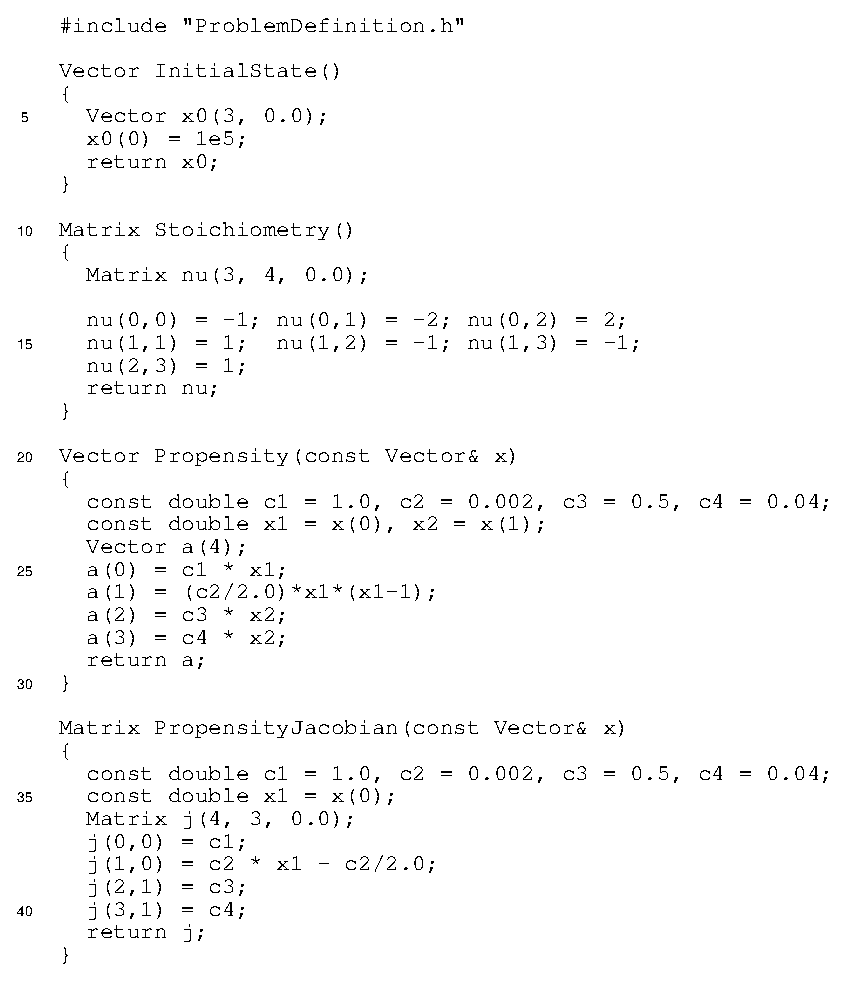
\includegraphics{dimer_decay_cpp.eps}
  \caption{Listing of \cpp\ test problem definition file
           \api{DimerDecayRxn.cpp}.}
  \label{testprob_cpp}
\end{figure}

The \api{Propensity()} and \api{PropensityJacobian()}
\footnote{The user does not always need this Jacobian function. The Jacobian
is only needed for implicit tau methods to solve stiff problems. } functions have
specific interface requirements due to the solver's dependence on
them.  Specifically, the \api{Propensity()} function expects to
receive a state vector \api{x} of dimension $N$ (the number of species),
and return  a propensity vector of dimension $M$ (the number of reaction channels).
Likewise, the \api{PropensityJacobian()} function expects to receive a
state vector \api{x} of dimension $N$ and return a Jacobian matrix of dimension
$N$ by $M$.

With all the details of our problem contained in a single file, we can
link it to single-realization and statistical endpoint sampling driver
programs at will.

\subsection{Generating a Single Realization}

With our test problem in place in file \api{DimerDecayRxn.cpp}, we
need a driver routine to exercise it.  In this section we will create
a driver routine that can generate a single realization of our test
problem using any of the supplied exact or accelerated methods.  The
driver file appears as Figure \ref{singletest_cpp}. It will be
helpful to refer to it as we discuss its structure.  We will refer to
the driver as \api{SingleDriver.cpp}.
\begin{figure}[htbp]
  \centering 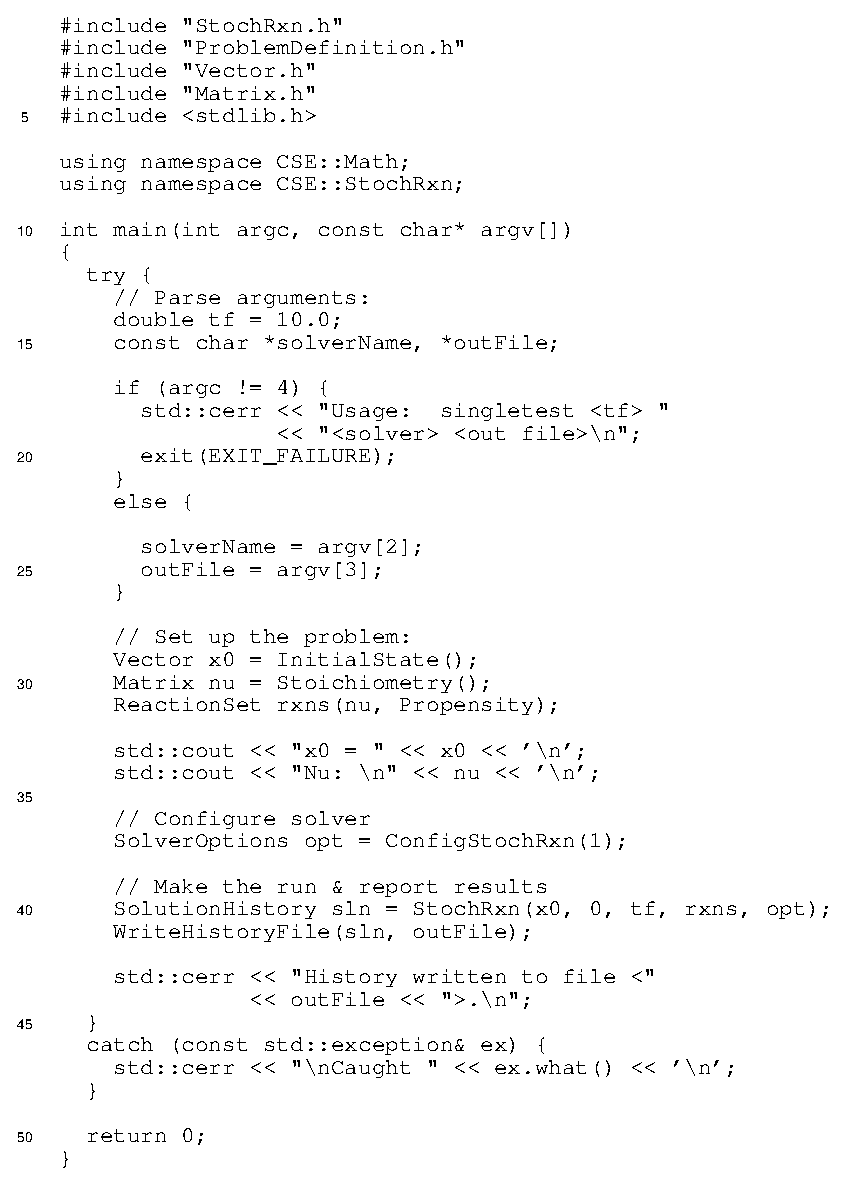
\includegraphics{singletest_cpp.eps}
  \caption{Listing of \cpp\ single-realization driver file
           \api{SingleDriver.cpp}.  The file is compatible with any
           problem defined according to \api{Prob\-lem\-Def\-ini\-tion.h}
           conventions.}
  \label{singletest_cpp}
\end{figure}

In lines 1--9 of the driver file, we include the necessary
declarations from the \stochrxn\ and CSE::MATH libraries.  In
particular, the functions defined in \api{DimerDecayRxn.cpp} are
declared in \api{ProblemDefinition.h} (line 2).  Lines 13--26 simply
parse the command line and set the
solver algorithm selection string (\api{solverName}) and output file
name (\api{outFile}) accordingly.  Lines 28--34 get the initial state
vector and stoichiometry matrix by calling the functions defined in
\api{DimerDecayRxn.cpp}.  A \api{ReactionSet} object is prepared in
line 31 to collect all the problem-specific information into a format
that the solvers understand.  Line 36 creates the \api{SolverOptions}
structure using the \api{ConfigStochRxn()} function. For users who are
only interested in an efficient SSA or tau-leaping solver, they do not
need to worry about the \api{SolverOptions}. For SSA, simply set
\api{SolverOptions opt = ConfigStochRxn(1);}. For tau-leaping method 
that automatically chooses $\tau$ value and switch to SSA when necessary, 
set \api{SolverOptions opt = ConfigStochRxn(1);}. For users who are
also interested in testing different formulas, they can modify these
options and get different results. Examples can be found in test 
directory. 

The call to the \api{StochRxn()} solver appears in line 40 of the
code.  The call returns a \api{SolutionHistory} object that contains a
single \api{SolutionPt} object containing time, population vector, and
selected stepsize information for each step made by the solver.  An
auxiliary function, \api{WriteHistoryFile()} is invoked after the
realization completes, to write the reaction history to a text file
readable by \matlab\ or any other program with plotting capability.
Finally, lines 46--51 handle error situations and cleanup.

To invoke the solver we compile both files and link them together and
with the \api{CSE\_Math} and \api{CSE\_StochRxn} libraries.  Assuming
we've named our executable file ``\srccode{dimersingle}'', a transcript of a
single run using the implicit \tauleaping\ solver follows:
\begin{code}
\begin{verbatim} 
dimersingle rxnhist.txt
x0 = [  1000  0  0  ]
Nu:
        -1      -2      2       0
        0       1       -1      -1
        0       0       0       1

History written to file <rxnhist.txt>.
\end{verbatim}
\end{code}
At the completion of this run, \api{rxnhist.txt} contains the time and
population vector data for each step, with one step per line.  This
file can be opened and plotted with \matlab.

\subsection{Generating an Endpoint Population Distribution}

\sspack \ was really designed with the generation of large
numbers of realizations in mind.  We can achieve this with a few small
modifications to the single realization driver code presented in
Figure \ref{singletest_cpp}.  The distribution generator code appears
in Figure \ref{stattest_cpp}. We will assume that it is stored in
source file \api{StatDriver.cpp}.
\begin{figure}[htbp]
  \centering \includegraphics{stattest_cpp.eps}
  \caption{Listing of \cpp\ multiple-realization driver file
           \api{StatDriver.cpp}.}
  \label{stattest_cpp}
\end{figure}

The main differences between the \api{StatDriver.cpp} and
\api{SingleDriver.cpp} files are highlighted here.  In line 1, we
include the \api{CollectStats.h} header file rather than the
\api{StochRxn.h} file.  An additional command-line parameter has been
added to capture the number of realizations to be performed, resulting
in the addition of lines 14 and 24.  Then, in lines 42 and 43, the
\api{CollectStats()} solver driver function is invoked, producing an
\api{EndPtStats} object that contains the final population vector for
each realization.  In line 45, these endpoint population vectors are
written to the specified text file via the \api{WriteStatFile()}
auxiliary function, one realization to a line.

Having prepared the distribution generator driver, we compile and link
as before.  Assuming that we create an executable named
\api{dimerdist}, a $10,000$ realization ensemble run would appear as follows:
\begin{code}
\begin{verbatim}
dimerdist 10000 endpts.txt
x0 = [  1000  0  0  ]
Nu:
        -1      -2      2       0
        0       1       -1      -1
        0       0       0       1

Run 10000 of 10000
Endpoints written to file <endpts.txt>.
\end{verbatim}
\end{code}
We will explain in Section \ref{dataanalyzer} how to
draw plots based on the ensemble data.

\subsection{Test Problems}
We have provided two simple test problems from the literature. One is the
the Dimerdecay problem studied in \cite{Gillespie01}, which
consists of three species $S_1,S_2$ and $S_3$ and four reaction channels:
\begin{equation}
\begin{aligned}
S_1 &\overset{c_1}{\rightarrow} 0 \\
S_1 + S_1 &\overset{c_2}{\rightarrow} S_2 \\
S_2 &\overset{c_3}{\rightarrow} S_1 + S_1\\
S_2 &\overset{c_4}{\rightarrow} S_3.
\end{aligned}
\label{eq_decay_dimeriz}
\end{equation}
The propensity functions are given by
$$
a_1 = c_1x_1, \quad a_2 = \frac{c_2}{2} x_1 (x_1-1), \quad a_3 = c_3 x_2, \quad a_4 = c_4 x_2,
$$
Following \cite{Gillespie01}, we chose values for the parameters
$$
c1 = 1.0, \quad c2 = 0.002, \quad c3 = 0.5, \quad c4 = 0.04.
$$
The initial conditions were changed to $x_1(0)=1000$, $x_2(0)=0$ and $x_3(0)=0$,
and the problem was solved on the time interval $[0, \ 10]$.

The second example is the Schl\"ogl reaction.
This reaction is famous for its bistable distribution.
The reactions are given by
\begin{equation}
\begin{array}{c}
B_1 + 2 X \underset{{c_2 }}{\overset{{c_1}}{\rightleftharpoons}} 3X, \\
B_2  \underset{{c_4 }}{\overset{{c_3}}{\rightleftharpoons}} X,  \\
\end{array}
\end{equation}
where $B_1$ and $B_2$ denote buffered species whose respective molecular
populations $N_1$ and $N_2$ are assumed to remain essentially constant
over the time interval of interest. Let
\begin{equation}
x(t) = \mbox{number of } X \mbox{ molecules in the system at time }t.
\end{equation}
The state change vectors are $\nu_1 = \nu_3 = 1$, $\nu_2 = \nu_4 = -1$. The propensity functions are
\begin{equation}
\begin{array}{rcl}
a_1(x) & = & \frac{c_1}{2} N_1 x (x - 1) , \\
a_2(x) & = & \frac{c_2}{6} x (x -1 ) ( x - 2), \\
a_3(x) & = & c_3 N_2 , \\
a_4(x) & = & c_4 x .
\end{array}
\end{equation}
For some parameter values, this model has two stable states. The parameter set that we used in our simulation has this property, and was given by
\begin{equation}
\begin{array}{c}
c_1 = 3\times 10^{-7}, \quad c_2 = 10^{-4}, \quad
c_3 = 10^{-3}, \quad c_4 = 3.5, \\
N_1 = 1 \times 10^5, \quad N_2 = 2 \times 10^5.
\end{array}
\end{equation}
We set the simulation interval from $t = 0$, with initial state $x(0) = 250$, to time $T = 4$.
Plots of different trajectories are shown in Figure \ref{schlogl_trajectory}
\begin{figure}[htbp]
  \centering 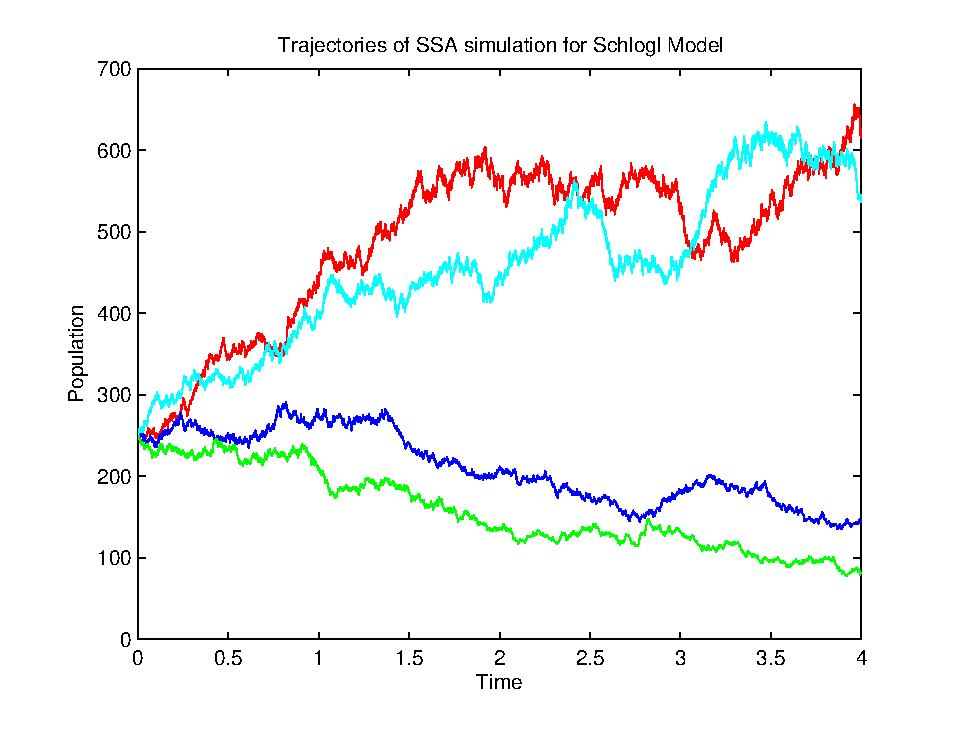
\includegraphics{schlogl_trajectory.eps}
  \caption{Different trajectories for the Schl\"ogl model.}
  \label{schlogl_trajectory}
\end{figure}

\section{Tools}
\subsection{Data Analyzer} \label{dataanalyzer}
The data analysis in deterministic simulation usually gives a trajectory of
the system states from the initial time to the final time. In stochastic
simulation, that can also be done. But of more relevance in the stochastic
simulation are the statistical properties. By repeating stochastic simulation
for many times with different random number sequences, we obtain an ensemble of the
data. The histogram can be plotted from the ensemble which represents the probability
density function of the corresponding variable. The cumulative distribution function
can also be plotted from the ensemble. In the tools directory, three \matlab\
subroutines are provided for plotting distributions.

A question that often arises in the research of stochastic simulation is how to measure
the error of the stochastic simulation. One may compare the ensemble from
the simulation with the ensemble from the experimental data, or compare it with
the ensemble from an ''exact'' simulation such as SSA. In either way, the answer
requires calculation of the distance between two distributions.
A number of distribution
distances have been proposed in the literature. In this package we provide three functions
to calculate two distribution distances. One is the total variance distance, which is
related to the histogram, defined as
\begin{equation} \label{d_distance}
        D(X, Y) = \int | p_X(s) - p_Y(s) | ds,
\end{equation}
where $p_X$ and $p_Y$ are the probability density functions of $X$ and $Y$ respectively.
Another is the Kolmogorov distance, which is related to
the cumulative distribution function, defined as
\begin{equation}
        K(X, Y) = \max_{-\infty < x < \infty} |F_X(x) - F_Y(x)|,
\end{equation}
where $F_X$ and $F_Y$ are the distribution functions of $X$ and $Y$ respectively
\footnote{
Note that the distribution function and the probability density function have
the relationship:
\begin{equation}
    F(x) = \int_{-\infty}^x p(s) ds.
\end{equation} }.
The details of the provided functions are listed below:

\begin{description}
\item[histoplot\_int] is a histogram plot subroutine which takes a vector as the first argument.
It assumes that the vector elements are integers. If a real-valued  vector is given, that
vector will automatically be rounded to integers. The probability for a variable to be
at a particular value (integer) is given by
the number of samples, whose value is equal to that integer,
divided by the total number of samples. The plot gives the calculated
probabilities for all the possible values. The mean, variance and standard deviation are
also calculated for the variable.


\begin{figure}
\begin{center}
\epsfxsize = 4in
\epsffile{dimerdistribution.eps}
\caption{   \label{dimerdistribution}
Histoplot\_int plot for $X_1$ in the Dimerdecay example. This plot is based on $10,000$ samples. }
\end{center}
\end{figure}

\begin{figure}
\begin{center}
\epsfxsize = 4in
\epsffile{schloglintdistribution.eps}
\caption{   \label{schloglintdistribution}
Histoplot\_int plot for Schl\"ogl example. This plot is based on $10,000$ samples. Note
    that because the values have a large range, this plot exhibits a large fluctuation.
}
\end{center}
\end{figure}

\item[histoplot\_real] is a histogram plot subroutine which takes a vector as the first argument,
and a positive integer as the second argument. The positive integer $K$ is the number of bins. Since
we do not assume that the vector contains only integers, bins are used to measure the histogram.
The bins are constructed by dividing the whole interval into $K$ subgroups (bins).
The probability that a random variable falls into a bin is the number of samples which are in
that bin divided by the total number of samples. The plot gives the calculated
probabilities for all the bins. The mean, variance and standard deviation are
also calculated for the variable.

\begin{figure}
\begin{center}
\epsfxsize = 4in
\epsffile{schlogldistribution.eps}
\caption{   \label{schlogldistribution}
Histoplot\_real plot for Schl\"ogl example. This plot is based on $10,000$ samples. The
    default number 50 of bins is applied.
}
\end{center}
\end{figure}

\item[cdfplot] is a cumulative distribution function (cdf) plot subroutine which takes a vector as the
first argument. The cdf value is calculated as the number of samples that are smaller than a
particular value, divided by the total number of samples. Here we do not distinguish whether the input
vector are integers. The mean, variance and standard variance are
also calculated for the variable.

\begin{figure}
\begin{center}
\epsfxsize = 4in
\epsffile{schloglcdf.eps}
\caption{   \label{schloglcdf}
cdfplot plot for the Schl\"ogl example. This plot is based on $10,000$ samples. }
\end{center}
\end{figure}

\item[histodistance\_int] calculates the histogram distance between two random variables. The first two
arguments are the vectors of the samples of two random variables. The numbers of samples (sizes of
the two vectors) do not have to be equal. It assumes that the two vectors contain integers. If not,
they will automatically be rounded to integers. The distance calculates the sum of the absolute value
of the difference between the calculated probabilities of the two ensembles. Since all data are integers,
the probabilities are calculated for integer values rather than bins.

\begin{figure}
\begin{center}
\epsfxsize = 4in
\epsffile{schloglintdifference.eps}
\caption{   \label{schloglintdistance}
histodistance\_int plot for the Schl\"ogl example. This plot is based on
$10,000$ samples of SSA runs and
explicit tau-leaping runs with tau = 0.4. }
\end{center}
\end{figure}

\item[histodistance\_real] calculates the histogram distance between two random variables. The first two
arguments are the vectors of the samples of two random variables. The numbers of samples (sizes of
the two vectors) do not have to be equal.
The third argument is a positive integer representing the number of bins.
Here we do not assume the data are integers. Thus the probabilities are calculated based on bins.
The rest is the same as the function histodistance\_int.

\begin{figure}
\begin{center}
\epsfxsize = 4in
\epsffile{schloglrealdifference.eps}
\caption{   \label{schloglrealdistance}
histodistance\_real plot for the Schl\"ogl example.
This plot is based on $10,000$ samples of SSA runs and
explicit tau-leaping runs with tau = 0.4. The
    default number 50 of bins is applied. }
\end{center}
\end{figure}

\item[kolmogorovdistance] calculates the Kolmogorov distance between two random variables.
The first two arguments are the vectors of the samples of two random variables. The numbers of samples
(sizes of the two vectors) do not have to be equal. The Kolmogorov distance measures the maximum
distance between the measured cdfs between the two random variables.


\begin{figure}
\begin{center}
\epsfxsize = 4in
\epsffile{schloglkolmogorovdifference.eps}
\caption{   \label{schloglkolmogorovdistance}
Kolmogorov distance plot for the Schl\"ogl example. This plot is based on
$10,000$ samples of SSA runs and
explicit tau-leaping runs with tau = 0.4. }
\end{center}
\end{figure}

\end{description}

\subsection{MPI Parallel Toolbox}
Monte Carlo simulation is naturally suited to parallel computation. In
\sspack \ we provide an MPI toolbox which enables users to parallelize
the collection of Monte Carlo ensembles. Although it is part of
the \sspack\ package, the application of this toolbox is not limited
to \sspack. Any Monte Carlo ensemble collection software can be parallelized after
small modifications to its code. To use this toolbox, simply follow these steps.

\begin{enumerate}
\item Set the environment variables to include the path for MPI.

{\it
Example: \\
setenv PATH \{\$PATH\}:/usr/local/mpich/bin/:.
}

\item  Compile \sspack. It is important to correctly compile \sspack \ for parallel computation.
We recommend using SPRNG to generate the random numbers
since it provides better performance and accuracy in random number generation on a parallel
machine. If you choose not to use SPRNG, we made our best efforts to avoid statistical error
due to the correlation between random number generation on different nodes. The results are still
quite trustable. If you choose to use SPRNG, please follow the README for SPRNG
(see under StochKit/Math/sprng2.0 or visit their website) to ensure that SPRNG is using its parallel
version. After you recompile SPRNG, you need to recompile \sspack. This step is important
to reduce the statistical error due to the correlation between random number generation
on different nodes.

\item Write the parallel code using our template. We will use the Dimerdecay model
as the example to explain this step. There are two other examples: the heatshock and Schl\"ogl
models under the directory "test". \footnote{Note: the directories starting with 'p'
are directories for parallel computing. Otherwise, they are for single processor systems.}
Suppose you have written your code for a single processor system. Copy all the files
for the single processor system to a new directory. Make the following changes.
\begin{enumerate}
\item Change your main function to a normal function call.

{\it
Example: (DimerDecay) \\
Open DimerStats.cpp.
Use "int DimerStats(int iterations, char* outFile)" to replace
the "main" fucntion line. Remove those lines concerned with the arguments and output file.
}

\item Update the include files to reflect the above change.

{\it
Example: \\
Put "int DimerStats(int iterations, char* outFile);" int DimerStats.h and
include DimerStats.h in DimerStats.cpp.
}

\item Copy parallel.cpp to the new directory and edit it as follows:
  \begin{enumerate}
   \item Add the include file for the new problem. \\
{\it
Example:    Add \\
\#include "Random.h" \\
\#include "DimerStats.h" \\
in parallel.cpp.
}

   \item Set parameters. These parameters are the following:

    \begin{enumerate}
    \item TotalIte:   How many samples you need to simulate.
        \item NodeIte:    How many samples each node will simulate at one assignment. This
        parameter should be chosen not be too small otherwise the message
        passing overhead will be large. Nor should it be too large,
        otherwise it may take too long for a slow node.
        \item ModelName: the directory name for the result.
    \end{enumerate}

{\it
Example: \\
          int TotalIte=10000; // We need an ensemble of 10000 samples \\
          int NodeIte=500;   // Each time, a node will simulate 500 samples \\
          char ModelName[50] = "DM"; // The name of this model
}

      \item Set the function to call. In the function
        "static unit\_result\_t do\_work(unit\_of\_work\_t work)",
    add your function call with work and workdir as parameters
    after the line \\
{\it
sprintf(workdir, "./result/\%d\%s/\%d.txt",
               myrank, ModelName, CalledTimes); }

         {\it
         Example: \\
              DimerStats(work, workdir); }
    \end{enumerate}

   \end{enumerate}

\item Copy the Makefile to your new directory and edit it as follows:
      \begin{enumerate}
    \item Set the EXE to the name you prefer for your code.

    {\it
         Example: \\
           EXE     = p\_dimer
    }
      \item Change parameters in the OBJS to the file name you use.

    { \it
         Example: \\
         OBJS = parallel.o DimerStats.o ProblemDefinition.o
    }
    \item Change other names for your model.
    \end{enumerate}

\item Compile the parallel code. Type "make clean" then type "make". Now you are ready to run
    the parallel code.

\item To run the parallel code, use the command "mpirun -np 8 p\_dimer (change it for your own model)".
      This means we will use 8 nodes to run the job. One will be the master node. Seven slave
    nodes will do the real simulation (this number has to be larger than 1).
   After the simulation is finished, you can find all the results in the directory "result".
   You can go to the subdirectory "result" to collect all the data. Just type "cat */* $>$result.txt".
    This UNIX command will save all the results in the file result.txt. \\
\end{enumerate}

{\bf NOTE}: Before and after your simulation, make sure
    that you have an empty directory "result". This will help to avoid mixing your simulation
    results.

Here are the CPU time statistics for the heatshock example using $16$ nodes on the CISE/IGERT cluster
in UCSB. The total number of samples is 10,000. Each subtask has 100 samples. The
CPU time statistics are:

\begin{center}
Node 1 working time: 65300.751900s \\
Node 2 working time: 71237.403293s \\
Node 3 working time: 71925.680539s \\
Node 4 working time: 72152.520430s \\
Node 5 working time: 72039.307552s \\
Node 6 working time: 64859.650003s \\
Node 7 working time: 72277.642849s \\
Node 8 working time: 71807.694310s \\
Node 9 working time: 72953.922793s \\
Node 10 working time: 73102.471573s \\
Node 11 working time: 62843.083589s \\
Node 12 working time: 73094.701832s \\
Node 13 working time: 72377.459407s \\
Node 14 working time: 72125.499277s \\
Node 15 working time: 64139.769542s \\

Total working time: 1052237.558889s   \\
\end{center}

\subsection{SBML2StochKit Converter}

SBML (System Biology Makeup Language) \cite{sbml}
is a computer-readable format for representing models of biochemical reaction networks. SBML
is applicable to
metabolic networks, cell-signaling pathways, regulatory networks, and many others.
Dozens of software packages
support this format. Many biochemical problems are written as SBML files. For the
convenience of SBML users, we provide an easy SBML to \sspack\  Converter using Java.
Here we explain how users can
translate an SBML file into the input files that \sspack\ needs.

\begin{enumerate}
\item  Prepare the SBML file of your model. Our converter accepts standard Version 1
(level 1 and 2) and Version 2 SBML files with some
additional requirements.
These requirements are
\begin{enumerate}
\item In the tag $<$listOfSpecies$>$, give the initial amount for each species.

{\it
   Example: \\
     $<$specie name="S1" compartment="DimerDecay" initialAmount="1000" boundaryCondition="false" $>$
}

\item In the tag $<$listOfReactions$>$, specify the kinetic law for each reaction.

{\it
   Example: \\
     $<$kineticLaw formula="c1*S1"$>$
}

\item In the tag $<$kineticLaw formula="c1*S1"$>$, specify the values of the parameters.

{\it
   Example: \\

    $<$listOfParameters$>$ \\
      $<$parameter name="c1" value="1"$>$ \\
    $<$listOfParameters$>$
}

\end{enumerate}

\item Set the environment variables in your shell. For example, if you use Cshell,
add the following lines to your .cshrc or run them via command line.

{\it
%\begin{center}
     setenv XML\_HOME $<$StochKit\_directory$>$/tools/SBML2StochKit/

     setenv  LD\_LIBRARY\_PATH \$XML\_HOME/test: \$LD\_LIBRARY\_PATH
%\end{center}
}
\item Compile our Converter with the following command

{\it
   javac -classpath .:\$XML\_HOME/classes/XML.jar:\$XML\_HOME/classes/xerces.jar Converter.java
}

\item Run the Converter with the following command

{\it
%\begin{center}
   java -ms128m -mx256 -classpath .:\$XML\_HOME/classes/XML.jar:\$XML\_HO\\
    ME/classes/xerces.jar Converter test.xml 10 \\
%\end{center}
}
where "test.xml" is the file name of your SBML file and "10" is final time you want to simulate
your system to.

\end{enumerate}

We have provided some simple examples to demonstrate how to use the SBML2StochKit Converter.
Figures \ref{dimersbml}-\ref{dimersimulation} show the source files and the generated files.


\bibliography{StochKitUserGuide.bib}
\bibliographystyle{plain} %{unsrt}
\newpage

\begin{figure}[htbp]
\centering \includegraphics{DimerXml.eps}
\caption{The first page of the SBML file for the DimerDecay model }
\label{dimersbml}
\end{figure}

\begin{figure}[htbp]
\centering \includegraphics{DimerXml2.eps}
\caption{The second page of the SBML file for the DimerDecay model }
\label{dimersbml2}
\end{figure}


\begin{figure}[htbp]
\centering \includegraphics{ProblemD.eps}
\caption{The  problem definition file generated by the SBML2StochKit Converter:
         \api{ProblemDefinition.\cpp}.}
\label{dimerprolem}
\end{figure}


\begin{figure}[htbp]
\centering \includegraphics{Dimer.eps}
\caption{The simulation code generated by SBML2StochKit Converter:
         \api{Dimer.\cpp}.}
\label{dimersimulation}
\end{figure}

\newpage

\appendix

\section{\sspack\ Function Reference}

This section serves as a basic reference for the \sspack\ implementation
of each of the components presented in Section
\ref{routines}. The general signature (including parameter
and return types) for each class of functions is presented, along with
a description of the purpose of each parameter and the expected
semantics of functions of that class.  All functions in this section
are defined in the \srccode{CSE::StochRxn} namespace.

%\doublespacing

\begin{table}%[htbp]
  \begin{center}
    \caption{\cpp\ driver function reference} \label{cpp_driver_tab}
    \begin{tabular}{|p{0.75in}|p{0.5in}|p{1.125in}|p{2.625in}|}
      \hline
      Name & \multicolumn{3}{l|}{\textbf{StochRxn}} \\
      \hline
      Signature & \multicolumn{3}{l|}{
          \srccode{SolutionHistory StochRxn(x0, t0, tf, react, opt)}} \\
      \hline
      Parameters &  Name & Type & Description \\
      \cline{2-4}
                 &  \srccode{x0} & \srccode{Vector} &
                       Initial reactant species populations \\
                 &  \srccode{t0} & \srccode{double} &
                       Initial time \\
                 &  \srccode{tf} & \srccode{double} &
                       Final time \\
                 &  \srccode{react} & \srccode{ReactionSet} &
                       Reaction details (stoichiometric matrix, propensity
                       function, propensity Jacobian function) \\
                 &  \srccode{opt} & \srccode{SolverOptions} &
                       Options structure produced by a call to
                       \api{ConfigStochRxn} \\
      \hline
      Return Value & \multicolumn{3}{p{4.5in}|}{A \srccode{SolutionHistory}
                     object containing a number of \srccode{SolutionPt} objects
                     that depends on the integration time and history buffer
                     management routine specified in \srccode{opt}.}  \\
      \hline
      Purpose & \multicolumn{3}{p{4.5in}|}{Generate a single realization of the
                reaction system specified in \srccode{react} by propagating
                the system from state \srccode{x0} at time \srccode{t0} to
                time \srccode{tf} using the algorithms specified in
                \srccode{opt}.} \\
      \hline
      \hline
      Name & \multicolumn{3}{l|}{\textbf{CollectStats}} \\
      \hline
      Signature & \multicolumn{3}{l|}{
         \srccode{EndPtStats CollectStats(runs, x0, t0, tf, react, opt)}} \\
      \hline
      Parameters & Name & Type & Description \\
      \cline{2-4}
                 &  \srccode{runs} & \srccode{unsigned int} &
                       Number of Realizations to perform \\
                 &  \srccode{x0} & \srccode{Vector} &
                       Initial reactant species populations \\
                 &  \srccode{t0} & \srccode{double} &
                       Initial time \\
                 &  \srccode{tf} & \srccode{double} &
                       Final time \\
                 &  \srccode{react} & \srccode{ReactionSet} &
                       Reaction details (stoichiometry matrix, propensity
                       function, propensity Jacobian function) \\
                 &  \srccode{opt} & \srccode{SolverOptions} &
                       Options structure produced by a call to
                       \api{ConfigStochRxn} \\
                   \hline
      Return Value & \multicolumn{3}{p{4.5in}|}{An EndPtStats object containing a
                     the final state vector from each realization.} \\
      \hline
      Purpose & \multicolumn{3}{p{4.5in}|}{Generate \srccode{runs} realizations
                of the reaction system specified in \srccode{react} by
                propagating the system from state \srccode{x0} at time
                \srccode{t0} to time \srccode{tf} using the algorithms
                specified in \srccode{react}.  Only the final state vector
                from each realization is stored.} \\
      \hline
    \end{tabular}
  \end{center}
\end{table}

\begin{table}%[htbp]
  \begin{center}
    \caption{\cpp\ stepsize selection function reference} \label{cpp_stepsize_tab}
    \begin{tabular}{|p{0.75in}|p{0.5in}|p{1.125in}|p{2.625in}|}
      \hline
      Name  & \multicolumn{3}{p{4.5in}|}{\textbf{Fixed\_Stepsize}} \\
            & \multicolumn{3}{p{4.5in}|}{\textbf{SSADirect\_Stepsize}} \\
            & \multicolumn{3}{p{4.5in}|}{\textbf{Gillespie\_Stepsize}} \\
	    & \multicolumn{3}{p{4.5in}|}{\textbf{GillespiePetzold\_Stepsize}} \\ 
	    & \multicolumn{3}{p{4.5in}|}{\textbf{Cao\_Stepsize}} \\ 
      \hline
      Signature & \multicolumn{3}{l|}{
          \srccode{double \emph{Name}(x, a, a0, nu, tau, eps, j)}} \\
      \hline
      Parameters &  Name & Type & Description \\
      \cline{2-4}
                 &  \srccode{x} & \srccode{Vector} &
                       Current reactant species populations \\
                 &  \srccode{a} & \srccode{Vector} &
                       Current reaction propensities \\
                 &  \srccode{a0} & \srccode{double} &
                       Sum of current reaction propensities \\
                 &  \srccode{nu} & \srccode{Matrix} &
                       Stoichiometric matrix (number of species $\times$
                       number of reactions) \\
                 &  \srccode{tau} & \srccode{double} &
                       Previous stepsize ($t_i - t_{i-1}$) \\
                 &  \srccode{eps} & \srccode{double} &
                       Accuracy control parameter (for accelerated methods) \\
                 &  \srccode{j} & \srccode{Propensity\-Jacobian\-Func} &
                       Pointer to function that evaluates Jacobian of reaction
                       propensity vector \\
      \hline
      Return Value & \multicolumn{3}{p{4.5in}|}{A \srccode{double} indicating
                     the size of the next step to take ($dt$).  Thus, if we
                     are executing step $i$ at time $t_i$, $t_{i+1} =
                     t_i + dt$.} \\
      \hline
      Purpose & \multicolumn{3}{p{4.5in}|}{ Given information regarding the
                current system state and the previous stepsize, determine
                the size of the next step to take, using the following methods:} \\
      \cline{2-4}
              & \multicolumn{2}{l|}{Name} & Description \\
      \cline{2-4}
              & \multicolumn{2}{l|}{\srccode{Fixed\_Stepsize}} &
                Constant stepsize equal to that specified via the
                \srccode{``init\_step''} parameter in the \api{ConfigStochRxn()}
                call \\
              & \multicolumn{2}{l|}{\srccode{SSADirect\_Stepsize}} &
                Step to the next reaction time indicated by the direct
                SSA method \\
              & \multicolumn{2}{l|}{\srccode{Gillespie\_Stepsize}} &
                Take step according to the leap condition presented in
                \cite{Gillespie01} \\
      \hline
    \end{tabular}
  \end{center}
\end{table}



\begin{table}%[htbp]
  \begin{center}
    \caption{\cpp\ single stepper function reference} \label{cpp_singlestep_tab}
    \begin{tabular}{|p{0.75in}|p{0.5in}|p{1.125in}|p{2.625in}|}
      \hline
      Name  & \multicolumn{3}{p{4.5in}|}{\textbf{SSA\_SingleStep}} \\
            & \multicolumn{3}{p{4.5in}|}{\textbf{ExplicitTau\_SingleStep}} \\
            & \multicolumn{3}{p{4.5in}|}{\textbf{ImplicitTau\_SingleStep}} \\
            & \multicolumn{3}{p{4.5in}|}{\textbf{ImplicitTrapezoidal\_SingleStep}} \\
        & \multicolumn{3}{p{4.5in}|}{\textbf{TrapezoidalTau\_SingleStep}} \\
      \hline
      Signature & \multicolumn{3}{l|}{
          \srccode{void \emph{Name}(x, t, dt, a, a0, nu, pf, pjf, absTol, relTol, rxn,
                         p)}} \\
      \hline
      Parameters &  Name & Type & Description \\
      \cline{2-4}
                 &  \srccode{x} & \srccode{Vector} &
                       Current reactant species populations \\
                 &  \srccode{t} & \srccode{double} &
                       Current time \\
                 &  \srccode{dt} & \srccode{double} &
                       Current stepsize \\
                 &  \srccode{a} & \srccode{Vector} &
                       Current reaction propensities \\
                 &  \srccode{a0} & \srccode{double} &
                       Sum of current reaction propensities \\
                 &  \srccode{nu} & \srccode{Matrix} &
                       Stoichiometric matrix (number of species $\times$
                       number of reactions) \\
                 &  \srccode{pf} & \srccode{Propensity\-Func} &
                       Pointer to function that evaluates reaction propensity \\
                 &  \srccode{pjf} & \srccode{Propensity\-Jacobian\-Func} &
                       Pointer to function that evaluates Jacobian of reaction
                       propensity vector. \\
                 &  \srccode{absTol} & \srccode{double} &
                       Absolute tolerance for implicit methods) \\
                 &  \srccode{relTol} & \srccode{double} &
                       Relative tolerance for implicit methods) \\
		 &  \srccode{rxn} & \srccode{int} &
                       reaction index of occuring reaction for SSA methods) \\
		 &  \srccode{p} & \srccode{Vector} &
                       number of reactoins for all reaction channels for tau-leaping methods) \\
      \hline
      Return Value & \multicolumn{3}{p{4.5in}|}{None.  The system state vector
                     \srccode{x} is modified in place. } \\
      \hline
      Purpose & \multicolumn{3}{p{4.5in}|}{ Given the current state \srccode{x},
                       time \srccode{t}, and the stepsize \srccode{dt} suggested
                       by the chosen stepsize selection function, advance
                       \srccode{x} to time \srccode{t}$+$\srccode{dt}. } \\
      \hline
    \end{tabular}
  \end{center}
\end{table}


\begin{table}%[htbp]
  \begin{center}
    \caption{\cpp\ history buffer management functions} \label{cpp_history_tab}
    \begin{tabular}{|p{0.75in}|p{0.5in}|p{1.125in}|p{2.625in}|}
      \hline
      Name  & \multicolumn{3}{p{4.5in}|}{\textbf{Exponential\_StoreState}} \\
            & \multicolumn{3}{p{4.5in}|}{\textbf{NoHistory\_StoreState}} \\
            & \multicolumn{3}{p{4.5in}|}{\textbf{OneHertz\_StoreState}} \\
      \hline
      Signature & \multicolumn{3}{l|}{
          \srccode{void \emph{Name}(hist, solPt)}} \\
      \hline
      Parameters &  Name & Type & Description \\
      \cline{2-4}
                 &  \srccode{hist} & \srccode{Solution\-History} &
                       History buffer \\
                 &  \srccode{solPt} & \srccode{SolutionPt} &
                       Object containing current time, state vector, and stepsize
                       for possible insertion into the history buffer \\
      \hline
      Return Value & \multicolumn{3}{l|}{None.} \\
      \hline
      Purpose & \multicolumn{3}{p{4.5in}|}{ At the discretion of the selected
                function, adds the current time, state, and step size to the
                history buffer.  Actual behavior is as follows:} \\
      \cline{2-4}
              & \multicolumn{2}{l|}{Name} & Description \\
      \cline{2-4}
              & \multicolumn{2}{l|}{\api{Exponential\_StoreState}} &
                Stores all solution points in the buffer, doubling the
                buffer's size when its capacity is exceeded \\
              & \multicolumn{2}{l|}{\api{NoHistory\_StoreState}} &
                Stores only the final solution point in the buffer \\
              & \multicolumn{2}{l|}{\api{OneHertz\_StoreState}} &
                Stores solution points at approximately $\unitqty{1}{s}$
                (integration time) intervals, regardless of the stepsize
                choices made by the stepsize selection function.  Useful
                for shrinking output file size when using SSA \\
      \hline
    \end{tabular}
  \end{center}
\end{table}
\end{document}
